\documentclass[10pt, conference, compsocconf]{IEEEtran}
\usepackage{graphicx,url}
\usepackage{subcaption} 
\usepackage{verbatim}

\begin{document}

\title{Titulo do Artigo}

\author{\IEEEauthorblockN{
		Marcos Guibson, Fernanda Pires
	}
\IEEEauthorblockA{Laboratório de Pesquisa e Desenvolvimento em Tecnologias Edcuacionais (TinkTEd)\\
Escola Superior de Tecnologia-Universidade do Estado do Amazonas (EST/UEA) \\
Amazonas, Brazil\\
mgss.lic17, fpires@uea.edu.br
}
}

\maketitle
\begin{abstract}
Aqui vai ficar o abstract do artigo


\end{abstract}
\begin{IEEEkeywords}
	key words;
\end{IEEEkeywords}

\begin{abstract}
Aqui vai ficar o resumo do artigo
	
\end{abstract}

\begin{IEEEkeywords}
palavras chaves;

\end{IEEEkeywords}

\IEEEpeerreviewmaketitle

\section{Introdução}
%RESOLUÇÃO DE PROBLEMAS

Aqui sera a parte ada introdução

\section{Trabalhos relacionados} \label{sec:firstpage}

Nos últimos anos, \textit{serious game} têm sido desenvolvidos em diferentes campos do conhecimento, inclusive em Ciência da Computação, contudo, a maioria desses jogos limitam-se a aprendizagem de linguagens de programação, ou estimulo da lógica computacional. Apesar disso, trabalhos recentes como o de \cite{figueiredo2011wargrafos} apresentam jogos que abortam aspectos mais complexos da ciência da computação \cite{yang2016developing}.

 Seguindo a linha de pesquisa similar, o jogo \textit{As aventuras de Biguió} é um jogo educacional mobile com visão 2.5D e estilo Dungeon. O jogo tem como objetivo de auxiliar no processo de visualização de problemas computacionais complexos para estudantes de computação, e promover o desenvolvimento do Pensamento Computacional para o público em geral \cite{melo2019aventuras}.
 
 Já o jogo \textit{StarDust}, é um jogo no estilo \textit{puzzle} para plataformas móveis \textit{Android}, voltado para a aprendizagem e aplicação do conceito de caminho mínimo em grafo. O jogo apresenta uma uma aprendizagem implícita, que permite que o jogo não se limite ao público alvo de alunos de nível superior \cite{melo2019stardust}.
 
 Do mesmo modo como os trabalhos mencionados, \textit{GraphFarm} proporciona um ambiente para o desenvolvimento do Pensamento Computacional através da resolução das missões do jogo, bem como auxilia na visualização e abstração de problemas computacionais clássicos utilizando as características dos grafos. 
 

\section{Pensamento Computacional}

%TÁ IGUAL DO SBIE

%ADICIONAR WING E STANZIONE (2016) E RETIRAR WING (2008)
O Pensamento Computacional segundo \cite{wing2006computational} é considerada como uma habilidade fundamental para todos, sendo comumente utilizada como instrumento que auxilia na resolução de problemas, bem como na compreensão do comportamento humano, baseando-se nos conceitos fundamentais da ciência da computação. Desta forma, o pensamento computacional deveria estar atrelado a prática analítica das pessoas, assim como a leitura e a escrita estão presentes desde a infância \cite{de2018ecologic}. Estudos comprovam que o desenvolvimento das habilidades do Pensamento Computacional podem contribuir positivamente, em um âmbito geral, a capacidade de resolver de problemas \cite{goulart2019labirinto,de2018ecologic,alencar2019looking}.

O desenvolvimento do PC segundo a perspectiva de \cite{learning2015computational} significa aprimorar os quatro pilares fundamentais a ele associados: decomposição, reconhecimento de padrões, abstração e algoritmos, construindo uma sequencia de passos para a resolução de problemas. Ao decompor,fragmentamos problemas em partes menores. O Reconhecimento de Padrões é buscar por semelhanças entre as características do problema. A Abstração contempla aspectos que podem ser relevantes no problema, para facilitar sua resolução e o Algoritmo é uma sequência de passos finitas para elaborar uma solução \cite{ferreira2019uso}

Pesquisas apontam a grande importância da disseminação de métodos e técnicas que auxiliam no desenvolvimento do Pensamento Computacional, dentre elas destacam-se os jogos digitais em cenários educacionais, que vem se mostrando uma ferramenta que visar tornar o processo de aprendizagem mais atraente e divertida \cite{savi2008jogos}. Diante deste cenário, um dos objetivos do jogo \textit{GraphFarm} é o desenvolvimento do Pensamento Computacional. 

\section{Processo de Aprendizagem}

Objetos de aprendizagem digitais são elementos instrucionais que podem ser utilizados em diferentes contextos, sendo baseados nos conceitos da Ciência da Computação \cite{denning2009beyond}. No contexto educacional a motivação dos alunos é um importante desafio com que nos devemos confrontar, pois tem implicações diretas na qualidade do envolvimento do aluno com o processo de ensino e aprendizagem \cite{lourencco2010motivaccao}.
%ADICIONAR DEFESA DO CONSTRUCIONISMO DE PAPERT + LINGUAGEM LOGO

%REESCREVER ISSO POIS NÃO FAZ SENTIDO NENHUM
O jogo \textit{GraphFarm} tem como sua base teórica de aprendizagem o Construcionismo de Seymour Papert, no qual faz uso do computador como uma ferramenta essencial para o processo de aprendizagem \cite{papert1994maquina}. Essa metodologia utiliza a auto regulação da aprendizagem, onde o jogador tem a capacidade de construir e adquirir seu próprio conhecimento \cite{alencar2019looking}.

Na perspectiva de Papert , projetar os sentimentos e ideias anteriores é a chave para o aprendizado. Em um abordagem construcionista, Papert acredita que o indivíduo pode construir seu próprio ciclo de aprendizado autodirigido e interativo através de ferramentas ou mediações que melhor suportam a exploração do conteúdo abordado \cite{ackermann2001piaget}. Assim como na linguagem \textit{LOGO}(linguagem de programação visual para crianças desenvolvida em 1968), o jogo \textit{GraphFarm} proporciona ao jogador uma experiência na construção de seus conhecimentos através da resolução de desafios contidos em cada parte do jogo.

\section{O jogo \textit{GraphFarm}}

%ADICIONAR TEXTO INTRODUTORIO
Esta seção apresenta o jogo \textit{GraphFarm} que foi idealizado para estudantes de computação em sua formação acadêmica e para o publico em geral, com o propósito de auxiliar na visualização e abstração de problemas computacionais e promover o desenvolvimento do Pensamento Computacional de forma divertida. \textit{GraphFarm} é um jogo de estratégia, com características 2D de RPG, desenvolvido na \textit{engine} \textit{Unity}, a partir da linguagem de programação $C\# $.


\subsection{Processo de desenvolvimento}

%ADICIONAR O PROCESSO DE DESENVOLVIMENTO DO JOGO. DESCREVER TODAS AS ETAPAS
Nesta seção são apresentadas as etapas de desenvolvimento do jogo, bem como detalhes e informações a respeito de sua produção. As etapas do processo de desenvolvimento do jogo podem ser identificadas na Figura ~\ref{fig1} e são descritas a seguir.

\begin{comment}
	\begin{figure}[!htbp]
	\centerline{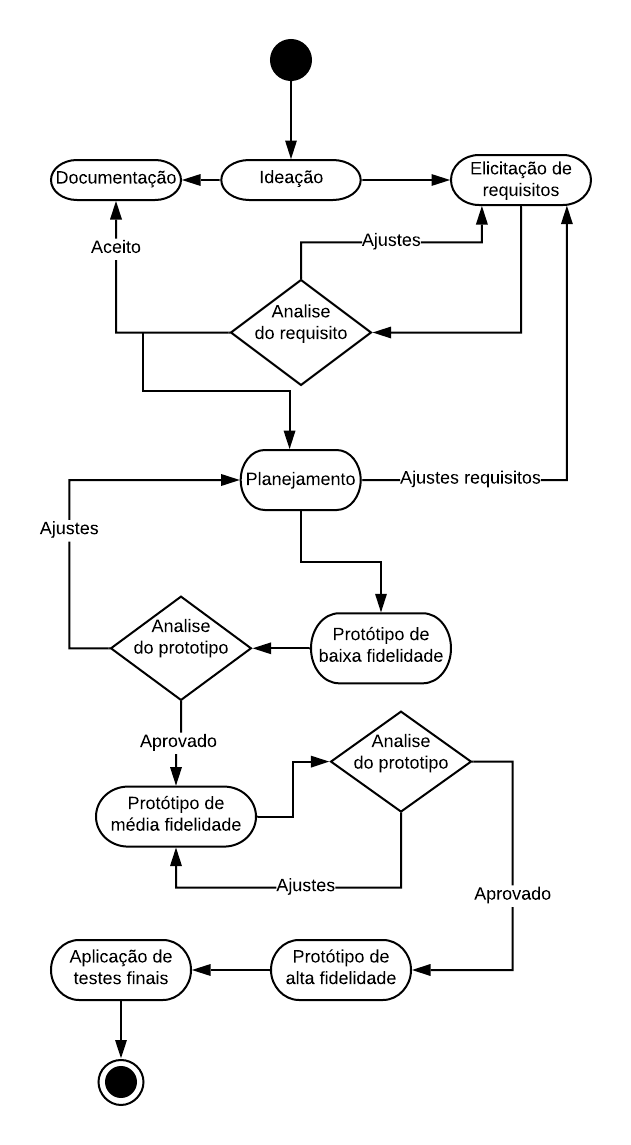
\includegraphics[scale=0.7]{Figuras/fig1.png}}
	\caption{Etapas de desenvolvimento.}
	\label{fig1}
	\end{figure}
\end{comment}



\begin{itemize}
	\item \textbf{Ideação:} nesta etapa foram concebidas as primeiras ideias para o jogo através de \textit{brainstorm}, incluindo a identificação das principais características e elementos do jogo, tal como a \textit{gameplay} e mecânica, além de iniciar os primeiros rascunhos para uma proposta visual para o jogo. No fim desta etapa foram definidas a personagem principal do jogo e suas características, a forma de recompensa e pontuação ao jogador utilizando estrelas para indicar o progresso de cada missão concluída, bem seu progresso durante as fases;
	

\begin{comment}
	\begin{figure}[!ht]
	\centering
	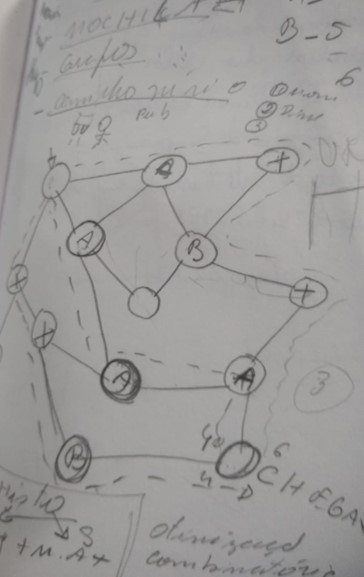
\includegraphics[width=0.4\linewidth]{Figuras/prototipo.jpg}		
	\caption{Primeiro rascunho do jogo.}
	\label{prototipo1}
	\end{figure}
\end{comment}	
	

	
	\item \textbf{Elicitação e análise de requisitos:} durante esta etapa foram levados os requisitos para o desenvolvimento do jogo, sendo eles funcionais e não funcionais, além dos aspectos pedagógicos que necessariamente deveriam contar no jogo. Durante o levantamento de requisitos foi discutida a garantia da auto regulação de aprendizagem no jogo, conduzindo o jogador a iniciar uma nova fase somente se a anterior estiver concluída, sempre aumentando a dificuldade da próxima fase. Os requisitos também passaram por uma análise gerando as funcionalidades e restrições. Foram necessárias novas discussões que resultaram em novos requisitos e adaptações dos requisitos anteriores. Dentre as novas mudanças, percebeu-se a necessidade de uma nova forma de controle da personagem principal do jogo;
	
	\item \textbf{Planejamento:} durante esta etapa foi realizada uma adaptação do \textit{Game Desing Document} (GDD). Nele são apresentadas informações detalhadas do jogo, tais como: descrição de elementos da \textit{gameplay} e mecânicas, características das fases, controles do jogador, sons e efeitos sonoros no ambiente, detalhes do \textit{heads-up display} (HUD) entre outras. Para um melhor entendimento dos elementos, optou-se por descrevê-la melhor na seção \ref{gdd};	

	\item \textbf{Protótipo de Baixa Fidelidade:} conhecidos como as primeiras rasuras dos jogos, são normalmente construídos com materiais diferentes da versão final, de forma simples e clara. Este tem por objetivo demostrar a ideia inicial do jogo, sendo considerado de fundamental importância nos estágios iniciais do desenvolvimento, pois trazem suporte à busca de alternativa de design e ideias. Durante esta etapa foi desenvolvido um pequeno modelo prévio de prototipagem visual do jogo, visando organizar os elementos nas telas e funcionalidades. O resultado desta etapa é um pequeno protótipo que representa as principais partes do jogo, bem como o formato de \textit{gameplay} e outros elementos importantes para mecânica, como controles, pontuação, objetivos e possíveis obstáculos. Nesta etapa foram realizados testes utilizando de usabilidade e experiência do jogador aplicando o MEEGA+ durante o SNCT(Semana Nacional de Ciência e Tecnologia) na Escola Superior de Tecnologia do Amazonas(UEA-EST) para alunos do núcleo de computação e tecnologia;
	
	

\begin{comment}
	\begin{figure}[!ht]
	\centering
	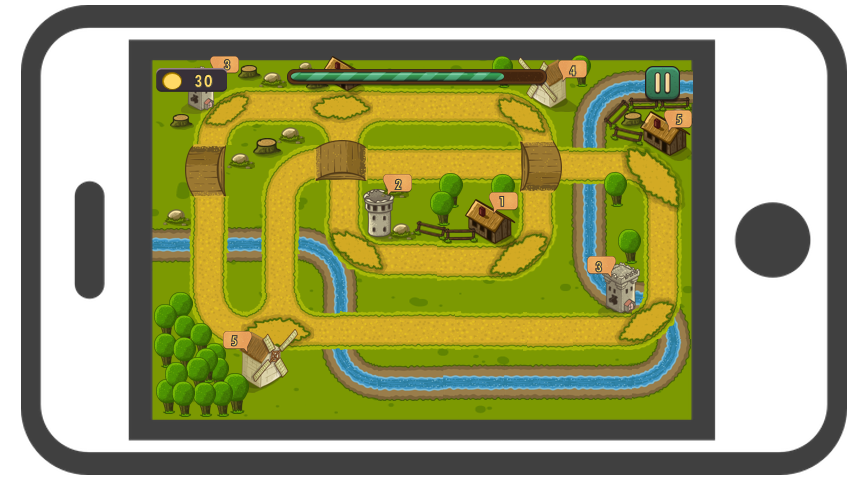
\includegraphics[width=0.8\linewidth]{Figuras/prototipo1.png}		
	\caption{Primeiro protótipo do jogo.}
	\label{prototipo1}
	\end{figure}
\end{comment}

	\item \textbf{Protótipo de Média Fidelidade:} o protótipo de média fidelidade seguiu as diretrizes presentes no GDD durante a implementação do jogo, executando conforme informações descritas na documentação. Durante esta etapa foi utilizado a \textit{ engine Unity} para a implementação. Como resultado desta etapa foi produzido um protótipo mais robusto, que serviu como base para o projeto final do jogo. O protótipo constou com a implementação das funcionalidades do jogo, bem como seus requisitos discutidos e definidos em etapas anteriores;
	

\begin{comment}
	\begin{figure}[!ht]
	\centering
	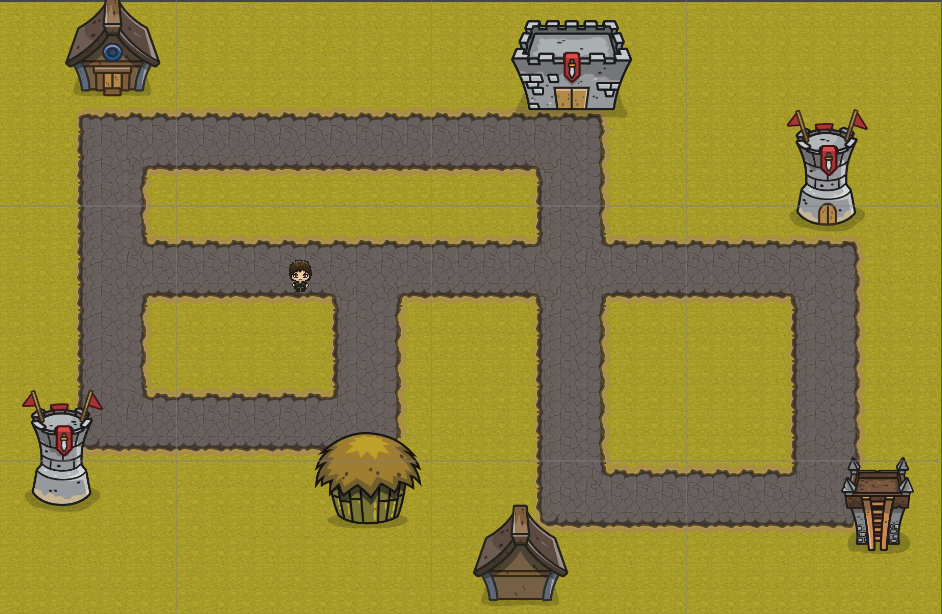
\includegraphics[width=0.8\linewidth]{Figuras/mediaFidelidade.png}
	\caption{Protótipo de media fidelidade.}
	\label{prototipo1}
	\end{figure}
\end{comment}

	\item \textbf{Protótipo de Alta Fidelidade:} o protótipo de alta fidelidade é a concepção que mais se assemelha com o produto que se prende a desenvolver, bem como consiste na implementação de melhorias no jogo. Nele estão implementadas todas as funções e alterações descritas na documentação e observadas nos testes iniciais dos protótipo de baixa e média fidelidade. Nesta etapa o jogo passou por novas mudanças em seu \textit{design} visual e disponibilidade para dispositivos  com sistema Androide.
	

\begin{comment}
	\begin{figure}[!ht]
	\centerline{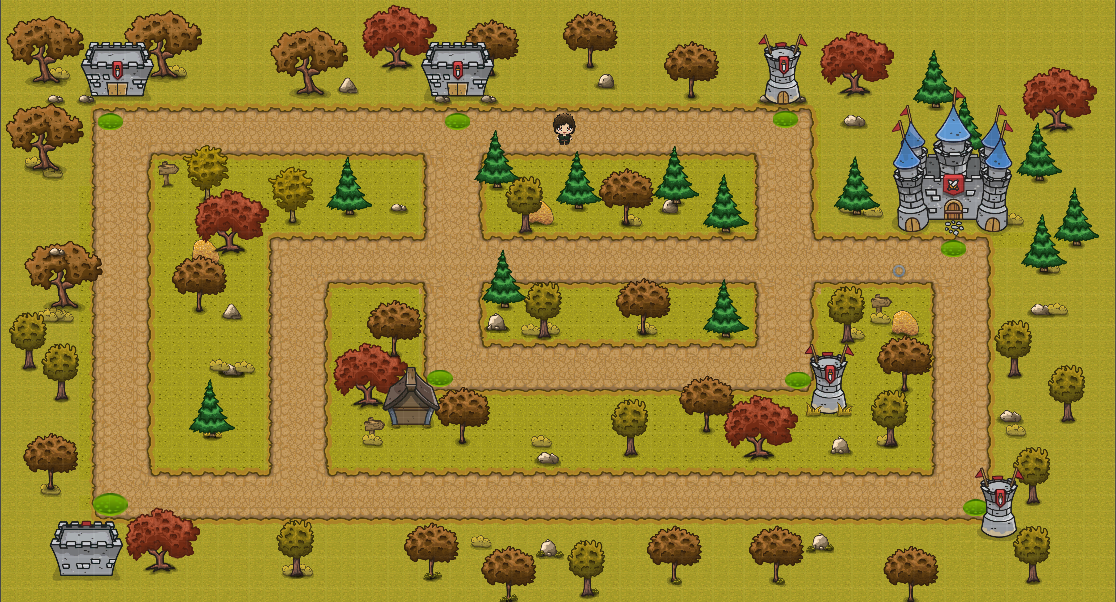
\includegraphics[width=0.8\linewidth]{Figuras/altaFidelidade.png}}
	\caption{Protótipo de alta fidelidade.}
	\label{prototipo3a}
	\end{figure}
\end{comment}
	
	\item \textbf{Validação de protótipo:} : a cada fim das etapas de protótipo de baixa, média e alta fidelidade, o aplicativo é avaliado para verificar se as funcionalidades implementadas estão de acordo com os requisitos definidos. A validação após protótipo de baixa e média fidelidade, foi realizada pelos desenvolvedores. Após o protótipo de alta fidelidade é realizada a avaliação das interfaces utilizando o Teste de Usabilidade de Nielsen \cite{nielsen1994usability} que também foi executado pelos desenvolvedores. Os resultados de cada validação de protótipo são utilizados para melhorar ou corrigir aspectos no jogo. Os resultados dos testes estão descritos na Seção \ref{resultado};
	

\begin{comment}
	\begin{figure}[!ht]
	\centering
	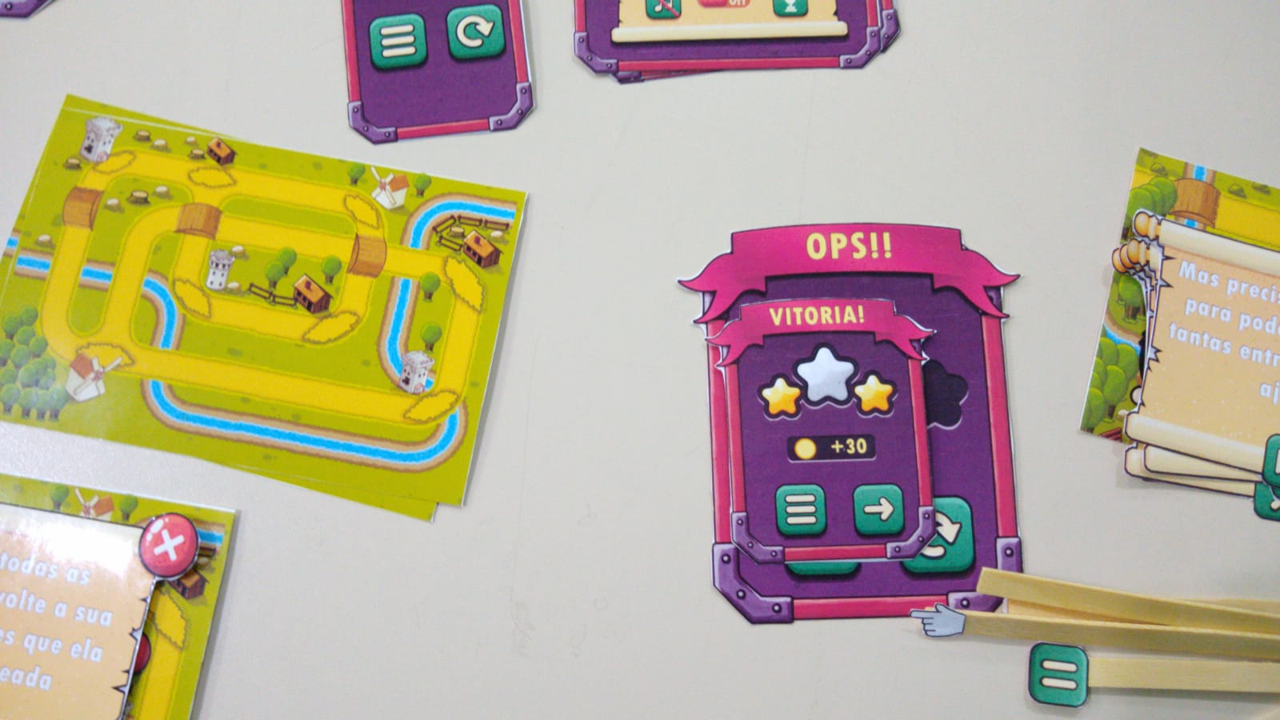
\includegraphics[width=0.8\linewidth]{Figuras/validacao.png}		
	\caption{Primeiro protótipo do jogo.}
	\label{prototipo1}
	\end{figure}
\end{comment}

	
	\item \textbf{Aplicação de testes finais:} nesta etapa são realizados testes com o usuário final. O aplicativo proposto é validado com usuários finais utilizando como forma de avaliação, o teste MEEGA+ \cite{von2018meega+}, que tem por objetivo avaliar os jogos com propósito educacional para aprendizagem de conceitos relacionados à computação. Os resultados dos testes apresentam as diferentes perspectivas dos usuários com relação ao jogo, tendo como ideia analisar as métricas de avaliação de cada usuário;
	
	\item \textbf{Documentação:} Durante todas as etapas do processo de desenvolvimento são gerados artefatos de documentação, entre eles o GDD. A documentação do projeto é composta de cronogramas do desenvolvimento, tornando-se assim, de grande importância para o projeto desde seu estado inicial, até o fim do seu ciclo de vida no encerramento do projeto. 
	

\begin{comment}
\begin{figure}[!htbp]
\centerline{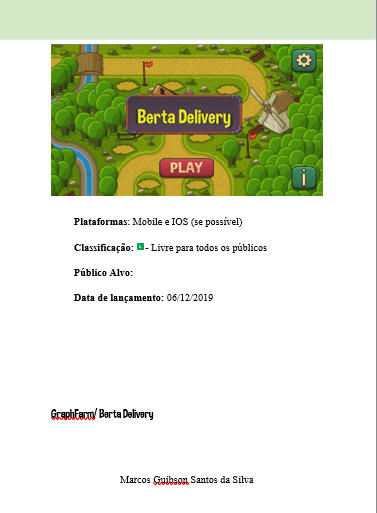
\includegraphics[scale=0.5]{Figuras/gddd.png}}
\caption{Game Design Document.}
\label{fig1}
\end{figure}
\end{comment}
	
\end{itemize}

\subsection{\textit{Game Design Document}} \label{gdd}
Game Design Document é um documento utilizado para registrar as principais etapas do desenvolvimento do jogo. O GDD conta com a descrição completa do jogo, a jornada do herói alinhada a jornada de conhecimento, bem como a disposição dos elementos de aprendizagem de acordo com os cenários do jogo, o storytelling, as mecânicas, a experiência de usuário, etc. 

\subsubsection{História}
A historia do jogo narra a história de Berta, uma jovem fazendeira que cuida de uma pequena fazenda ao norte do reino de Grafolandia. Em tempos de crise no reino, o rei solicita ajuda de Berta dos seus serviços de entregas para distribuir alimentos a população. O objetivo de Berta é realizar de maneira eficaz as missões que lhe são recebidas pelo rei.

\subsubsection{Fluxo do Jogo}
O \textit{GraphFarm} é um jogo de gênero \textit{Puzzle}, que abrange as noções de problemas computacionais clássicos utilizando as características de grafos, caracterizado pelo seu aspecto educacional, voltado para o desenvolvimento do pensamento computacional através da resolução de problemas. No jogo, os jogadores tem a função de ajudar Berta a combater a crise que se instalou no reino de GrafoLandia realizando entregas por todo o reino. O jogo é dividido em 4 fases distintas, cada uma com tempo limitado de jogo e suas características de cada tipo de missão passada pelo rei. A dificuldade nas transições entre fases é perceptível, a cada fase o grau de dificuldade aumenta gradativamente através de missões mais complexas e menos recursos dispostos ao usuário. O feedback ao jogador será medido de acordo com a eficácia da resolução de cada fase, se baseando na quantidade de passos, tempo estimado ou na qualidade da resolução do problema previamente estipulados.

\subsubsection{Mecânica}
Afim se ajudar o reino de GrafoLandia, o jogador deve propor uma forma de resolver o problema estipulado pelo jogo, ou seja, o jogador deve idealizar uma estratégia para a resolução das missões do jogo com base nos requisitos necessários para completar a missão. O jogador tem a seu dispor, a movimentação do personagem de acordo com os pontos de adjacência referentes ao local atual do jogador, sendo possível apenas se deslocar para os pontos no caminho que sejam conectados a posição atual do personagem. 


\subsubsection{Telas}\label{GDD}
A transição entre as telas pode ser visualizada no diagrama de telas, conforme ilustra Figura \ref{diagramaTelas}. É possível observar que, a partir do Menu Principal o usuário pode ir para Configurações, Seleção de Fases ou Informações. É importante destacar que, levando em consideração a carga cognitiva da aprendizagem, o usuário só pode selecionar fases já visitadas. Caso ele ainda não tenha passado de uma fase, esta não estará habilitada para visita do usuário.



\begin{comment}
	\begin{figure}[htbp]
	\centering
	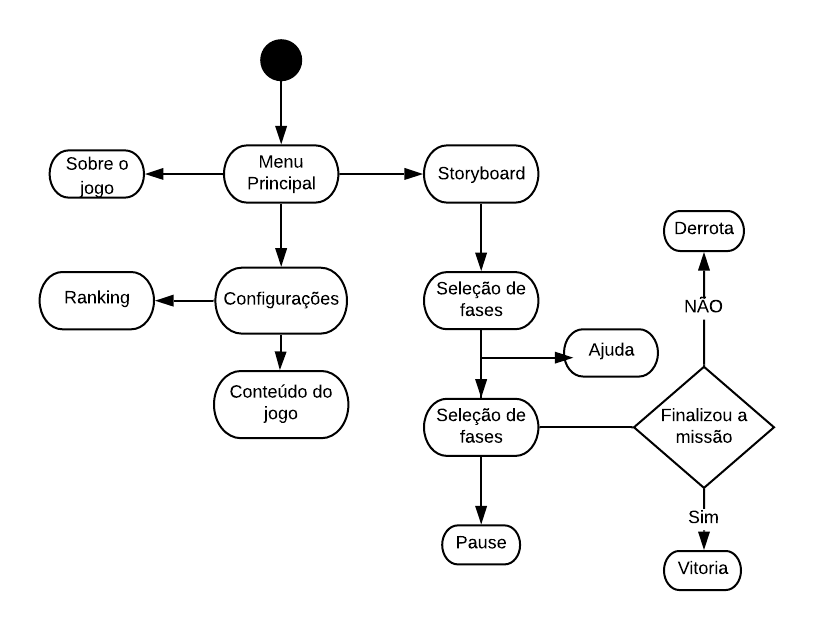
\includegraphics[width=.4\textwidth]{Figuras/Diagrama.png}
	\caption{Diagrama de telas.}\label{diagramaTelas}	
	\end{figure}
\end{comment}

\subsubsection{Fases}\label{GDD}
Cada fase do jogo possui um \textit{layout} individual, se diferenciando através do percurso do jogador para realizar duas missões com diferentes rotas. A figura \ref{fig9} ilustram a mecânica das três fases, sendo ela a fase tutorial do jogo. É possível observar que a Fase 1, que tem como objetivo apresentar o cenário do jogo e ambientar o jogador, tem um nível de dificuldade e possibilidade de movimentos menores, conforme ilustra a Figura \ref{faseTutorial}. As Figuras\ref{fase2} e \ref{faseFinal}, representam o cenário das fases seguintes, com uma maior quantidade de caminhos para a serem realizados, bem como uma novo \textit{design} dos níveis.



\begin{comment}
	\begin{figure}[ht]
	\centering
	\begin{subfigure}[b]{0.30\textwidth}
	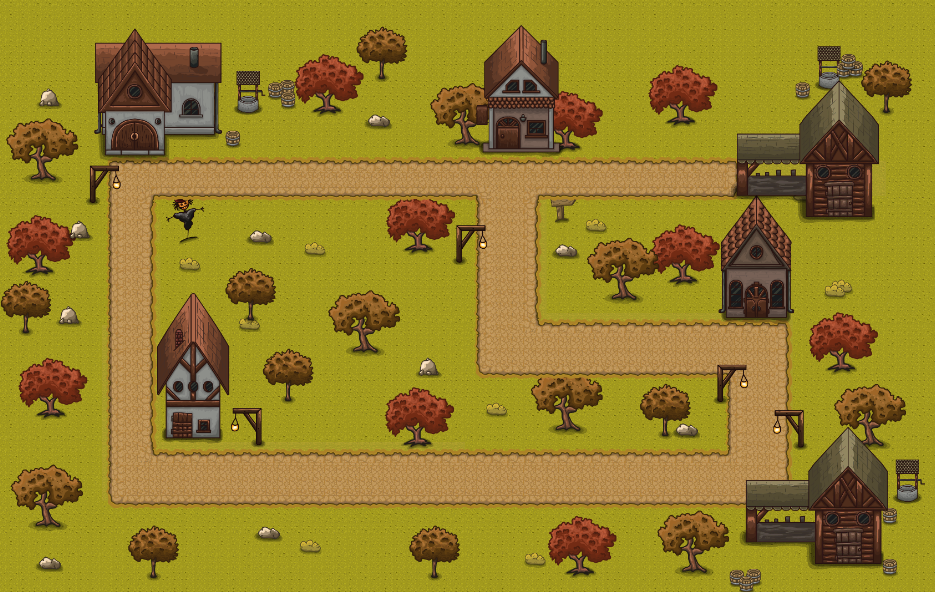
\includegraphics[width=\textwidth]{Figuras/faseTutorial.png}
	\caption{}
	\label{faseTutorial}
	\end{subfigure}
	
	\begin{subfigure}[b]{0.30\textwidth}
	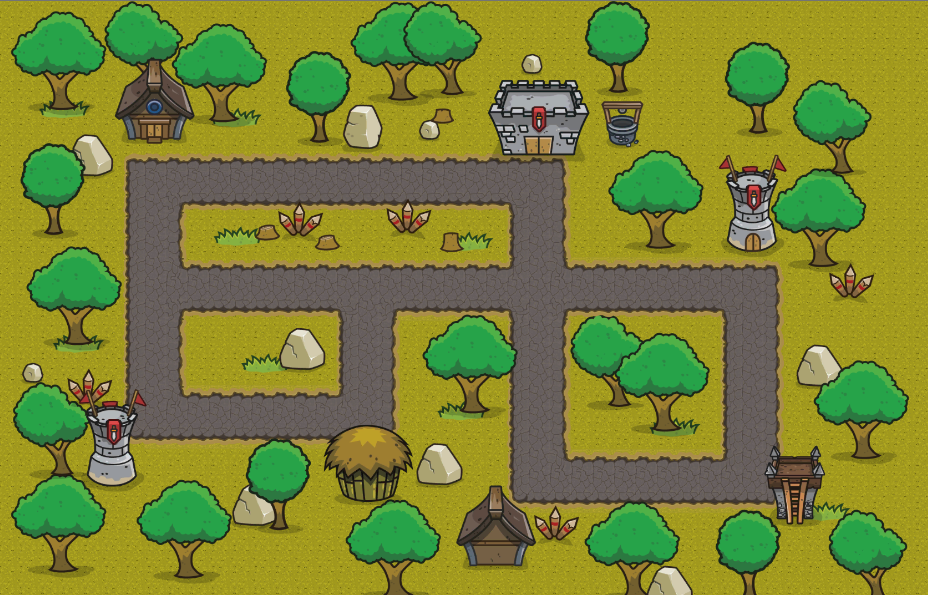
\includegraphics[width=\textwidth]{Figuras/fase2.png}
	\caption{}
	\label{fase2}
	\end{subfigure}
	
	\begin{subfigure}[b]{0.30\textwidth}
	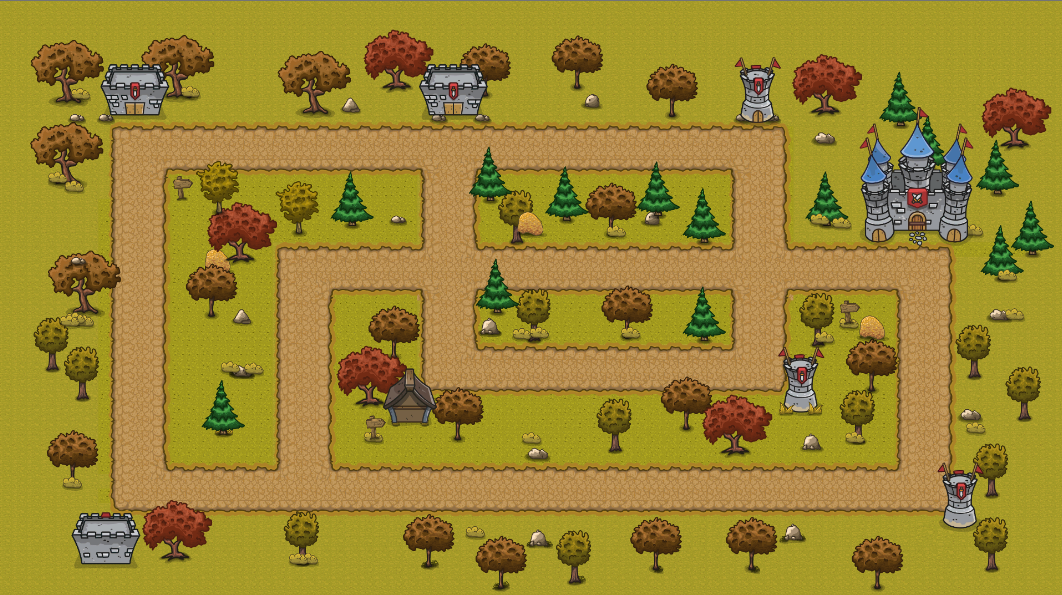
\includegraphics[width=\textwidth]{Figuras/fase3.png}
	\caption{}
	\label{faseFinal}
	\end{subfigure}
	
	\caption{(a) Fase tutorial. (b) Fase 1 – Problema da Mochila (c) Fase 2 – Caixeiro Viajante. } 
	\label{fig9}   
	\end{figure}
	
\end{comment}

\subsubsection{Controle} \label{GDD}
Os comandos para guiar a personagem principal do jogo serão realizados com os toques na tela realizados pelo jogador através do touch screen, dando ao usuário uma liberdade de movimentação pelo cenário dentro das limitações dos caminhos disponíveis pelo cenário. O jogador poderá mover o personagem através dos pontos de adjacências de acordo com a posição das interseções entre os caminhos.
Dependendo dos movimentos realizado pelo jogador, a personagem Berta pode realizar os seguintes movimentos:


\begin{comment}
	\begin{figure}[htbp]
	\centering
	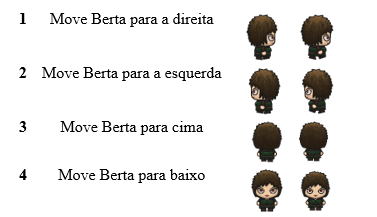
\includegraphics[width=.4\textwidth]{Figuras/controle.png}
	\caption{Movimentos da personagem.}\label{controlePersonagem}	
	\end{figure}
\end{comment}

\begin{comment}
		\begin{table}[!ht]
	\caption{Missões e objetivos do jogo \textit{GraphFarm.}}
	\begin{center}
	\begin{tabular}{|p{2.5cm}|p{4cm}|}
	\hline
	\textbf{Fases}&\textbf{\textit{Missões/Objetivo}} \\
	\hline
	Tutorial & 
	Fazer com que o jogador se acostume com a mecânica do jogo e realizar uma pequena busca de um item\\
	\hline
	Fase 1 – Pro. Mochila & Busque os ingredientes para o antidoto até o mestre de poções no castelo
	
	\\
	\hline
	Fase 2 – Caixeiro Viajante & 
	Realize todas as entregas e retorne a sua fazenda para evitar que ela seja saqueada.
	
	\\
	\hline
	Fase 3 – Fase final & 
	Sequencia de etapas para:
	Realize todas as entregas de leite no vilarejo antes que ele se estregue.
	
	\\
	\hline
	\end{tabular}
	\label{tab2}
	\end{center}
	\end{table}
	
\end{comment}

	
	


\begin{comment}	
\subsection{\textit{Algoritmo no jogo}}
	
			\subsection{Algoritmo no jogo: passo a passo}
		Para desviar de obstáculos, conquistar estrelas (pontuação) e resgatar os animais de cada fase é necessário construir a solução mais adequada para cada etapa do jogo. Como exemplo, a Figura ~\ref{fase3cresp} apresenta na imagem ~\ref{fase3}, a tela da Fase 3 do jogo, ilustrando antes de começar a partida  e uma possível solução para a Fase 3, na imagem ~\ref{fase3Resposta}. Após o jogador selecionar o conjunto de movimentos que representa a solução, este executa e caso esteja correto vai para a próxima fase, caso contrário volta para o início da fase atual.
		
		
		\begin{figure}[ht]
		\centering
		\begin{subfigure}[b]{0.45\textwidth}
		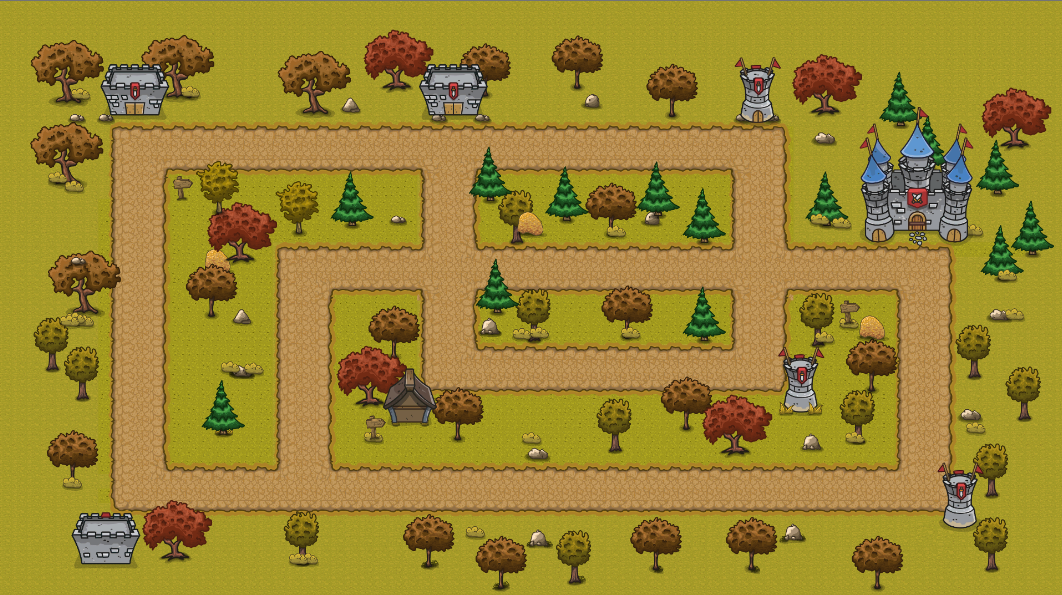
\includegraphics[width=\textwidth]{Figuras/fase3.png}
		\caption{}
		\label{fase3}
		\end{subfigure}
		
		\begin{subfigure}[b]{0.45\textwidth}
		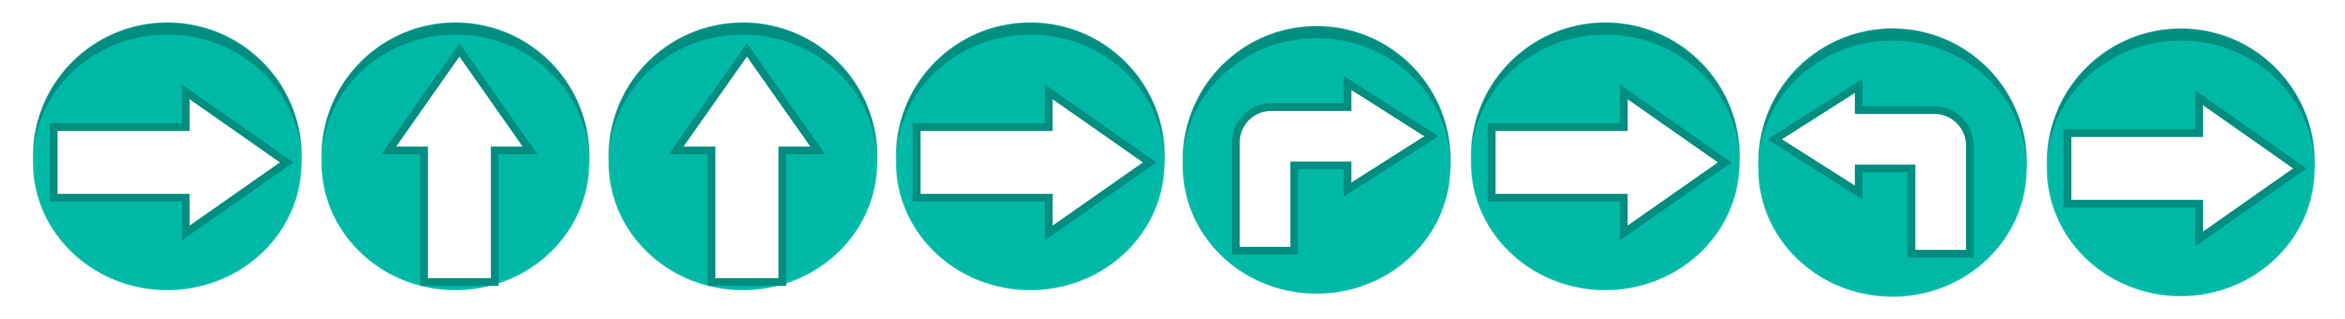
\includegraphics[width=\textwidth]{Figuras/fase3Resposta.png}
		\caption{}
		\label{fase3Resposta}
		\end{subfigure}
		\caption{(a) Fase 3 do Jogo. (b) Possível solução para a Fase 3. } 
		\label{fase3cresp}   
		\end{figure}
	\end{comment}
	


\begin{comment}
		\begin{table}[!ht]
	\caption{Tabela de critérios selecionados do MEEGA+.}
	\begin{center}
	\begin{tabular}{|l|p{5.8cm}|}
	\hline
	\textbf{Critérios}&\textbf{Descrição da avaliação} \\
	\hline
	Estética & Se a interface do jogo está agradável ao usuário. \\
	\hline
	Aprendizagem & Se o jogo pode ser utilizado pelo usuário para alcançar metas específicas de aprender a jogar com eficiência, satisfação e liberdade.
	\\
	\hline
	Controle & Se o jogo pode ser usado por usuários com problemas visuais.
	\\
	\hline
	Desafio & Se o jogo possui grau de dificuldade adequado ao desempenho do usuário.
	\\
	\hline
	Satisfação & Se os alunos sentem que o esforço no jogo resulta em algum tipo de aprendizado.
	\\
	\hline
	Diversão & Se o jogo promove sensações de prazer, felicidade, entretenimento e distração nos usuários.
	\\
	\hline
	Atenção & A atenção, concentração e foco.
	\\
	\hline
	Relevância & A relação da percepção dos usuários com a proposta educacional.
	\\
	\hline
	\end{tabular}
	\label{tab3}
	\end{center}
	\end{table}
	
\end{comment}	
	
	


\section{Resultados e Discussões} \label{resultado}
%FALAR SOBRE OS RESULTADOS E ANALISE DOS TESTES USANDO O MEEGA+ E O PROCESSO DE TRANSMISSÃO DO CONHECIMENTO USANDO O GAMIFICATION

Nesta seção será apresentada os tipos de testes realizados durante o processo de desenvolvimento do jogo. Para análise dos requisitos de aprendizagem, foram avaliados os elementos de objetos de aprendizagem \cite{alves2015gamification} e a experiência do jogador quanto a usabilidade utilizando o método MEEGA+ através a experiência causada no jogador \cite{von2018meega+}.

\subsection{Pensamento Computacional e o jogo}
%CRIAR SUBSEÇÃO: PENSAMENTO COMPUTACIONAL NO JOGO
O jogo busca exercitar as habilidades do Pensamento Computacional induzindo os jogadores a criarem soluções criativas através da construção de algoritmos. A Tabela \ref{tab2} apresenta a relação dos pilares do PC com aspectos do jogo.



\begin{comment}
	\begin{table}[!ht]
	\caption{Pensamento Computacional e \textit{GraphFarm.}}
	\begin{center}
	\begin{tabular}{|p{2.5cm}|p{5cm}|}
	\hline
	\textbf{Pensamento Computacional}&\textbf{\textit{GraphFarm}} \\
	\hline
	Decomposição & 
	Organizar os elementos e objetos em uma fase de maneira sistematizada\\
	\hline
	Reconhecimento de padrões & Organização espacial;
	
	Organização espacial;
	Distribuição dos elementos no jogo;
	Localização dos pontos;
	Formação de obstáculos;
	
	\\
	\hline
	Abstração & 
	Principais objetivos do jogo:
	
	- Formas de movimentação do personagem;
	
	- Objetivo da missão da missão;
	
	- Limitações das missões;
	
	\\
	\hline
	Algoritmo & 
	Sequencia de etapas para:
	
	- Realizar missões;
	
	- Coletar pontos;
	
	- Ser eficaz/eficiente;
	
	\\
	\hline
	\end{tabular}
	\label{tab2}
	\end{center}
	\end{table}
\end{comment}

\subsection{Analise de experiência do jogador}
Com o uso de uma das versões dos produtos do jogo (protótipo de média fidelidade),foram realizados os testes do MEEGA+, no qual propõe 12 categorias, sendo: Estética, Aprendizagem, Controle, Acessibilidade, Desafio, Satisfação, Interação Social, Diversão, Atenção Relevância, Confiança e Aprendizagem Percebida \cite{von2018meega+}.Como a proposta do jogo não aborda aspectos de acessibilidade e controle, estas categorias foram tiradas da avaliação.

A tabela \ref{Tab6} apresenta o resultado do teste do MEEGA+ aplicado ao jogo. Foram avaliados 10 critérios por 15 avaliadores em uma amostra de jogos realizados na SNCT (Semana Nacional de Ciências e Tecnologias) com alunos dos cursos de Computação e das Engenharias. O teste MEEGA+ foi utilizado avaliando em escalas entre 1 a 5, sendo: 1 = Não possui, 2 = Existem alguns, 3 = Suficiente, 4 = Bom e 5 = Ótimo.  




\begin{comment}
	\begin{table}[ht]
	\caption{Resultado da avaliação MEEGA+.}
	\begin{center}
	\begin{tabular}{|p{1.6cm}|p{.9cm}|p{.9cm}|p{.9cm}|p{.9cm}|p{.9cm}|}
	\hline
	\multicolumn{1}{|c|}{\textbf{Parâmetros}} & \textbf{Não possui
	} & \textbf{Existem alguns} & \textbf{Suficiente} & \textbf{Bom} & \textbf{Ótimo} \\ \hline
	
	Estética 
	& 0.0\% & 0.0\%    & 10.0\%     & 16.7\%   & 73.3\% \\ \hline
	
	Aprendizagem 
	& 0\% & 4.4\% & 22.2\% & 40.0\%  & 33.3\% \\ \hline
	
	Controle
	& 3.3\%   & 0.0\%   & 3.3\%    & 16.7\%  & 7.7\% \\ \hline
	
	Desafio 
	& 0.0\% & 2.2\% & 22.7\% & 17.8\%  & 57.8\% \\ \hline
	
	Satisfação 
	& 1.7\% & 1.7\% & 11.7\% & 21.7\% & 63.3\% \\ \hline
	
	Diversão 
	& 6.7\% & 0.0\% & 13.3\% & 23.3\%  & 56.7\% \\ \hline
	
	Atenção focada
	& 1.7\% & 1.7\% & 36.7\% & 16.7\%  & 43.3\% \\ \hline
	
	Relevância 
	& 2.0\% & 3.9\% & 27.5\% & 15.7\%  & 51.0\% \\ \hline
	
	Operabilidade 
	& 3.3\% & 0.0\% & 3.3\% & 16.7\%  & 76.7\% \\ \hline
	
	Confiança 
	& 0.0\% & 0.0\% & 26.7\% & 6.7\%  & 66.7\% \\ \hline
	\end{tabular}
	\end{center}
	\label{Tab6}
	\end{table}
\end{comment}

Durante o jogo, para que seja possível a conclusão das fases, o jogador deve realizar as missões presentes em cada nível. De acordo com o modo de como as missões foram realizadas, o jogador receberá seu feedback baseados em estrelas, quanto maior a quantidade de estrelas, melhor terá sido a resolução criada pelo jogador.
	
	
	
\subsection{Analise de Aprendizagem do jogo}	
%FALAR DO SAM e os resultados obtidos
O desenvolvimento do Self-Assessment Manikin (SAM) é utilizado para avaliar diretamente o prazer, a excitação e a dominância associada em reposta a um objeto ou evento, sendo inicialmente implementado como programa de computador interativo e posteriormente expandido para uma versão em papel para avaliarem grupos em massa. \cite{bradley1994measuring}. O teste da analise do SAM foi realizado através de uma plataforma \textit{mobile}, após os usuários terem acesso ao \textit{game}, levantando questionamentos sobre quais emoções foram despertadas ao jogador durante o processo de teste.
 
O SAM varia de um sorriso, figura feliz para uma figura infeliz e carrancuda quando representando a dimensão prazer e varia de uma figura animada e de olhos arregalados a uma pessoa relaxada, figura sonolenta para a dimensão da excitação. 



\begin{comment}
	\begin{figure}[htbp]
	\centering
	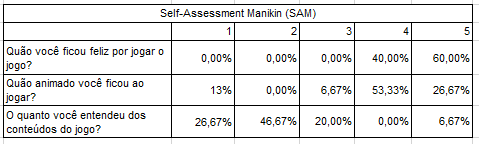
\includegraphics[width=.4\textwidth]{Figuras/sam.png}
	\caption{Measuring emotion (SAM).}\label{diagramaTelas}	
	\end{figure}
\end{comment}

\section{Considerações finais}
Aqui ficam as considerações finais  


\bibliographystyle{IEEEtran}
\bibliography{sbc-template}
\end{document}


